\documentclass{article}
\usepackage[UTF8,heading=true]{ctex}
\usepackage{graphicx}
\usepackage{ccaption}
\usepackage{minted}
\usepackage{url}
\usepackage[linkcolor=blue,
            CJKbookmarks=true,
            citecolor=blue,
            urlcolor=blue,
            colorlinks,
            pdfauthor={Marlin, <marlinhz@foxmail.com>}]
            {hyperref} %% pdf 结果文档属性.
\newcommand{\mt}[1]{\mintinline{tex}|#1|}
\begin{document}
\title{中英文图表标题测试}
\author{Marlin}
\maketitle	
	
需要给图形或表格等加双语标题时,可以重复使用caption命令。
在给出一种语言的标题后,将计数器 figure 减1,并重定义 figure。
\begin{minted}[xleftmargin=1cm]{tex}
\begin{figure}[htbp]
  \begin{minipage}{.5\linewidth}\centering
    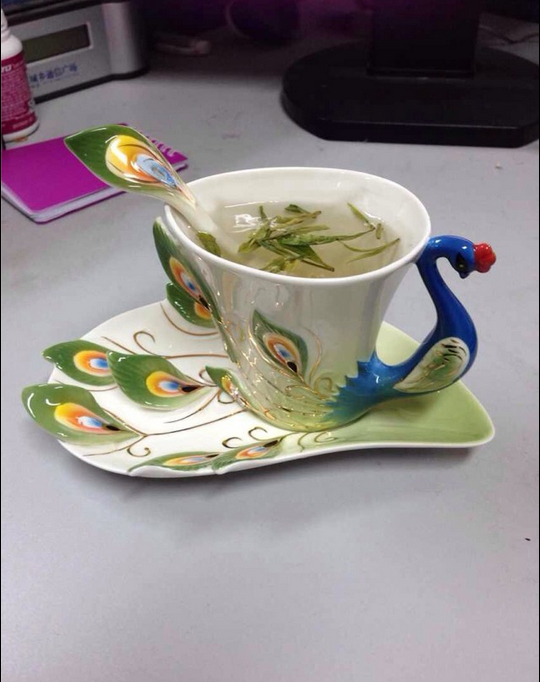
\includegraphics[width=.5\linewidth]{p1}
    \caption{中文标题}
    \addtocounter{figure}{-1}
    \vspace{-11pt}
    % Set English Caption
    \renewcommand{\figurename}{Fig}
    \caption{English title}
  \end{minipage}%
  \begin{minipage}{.5\linewidth}\centering
    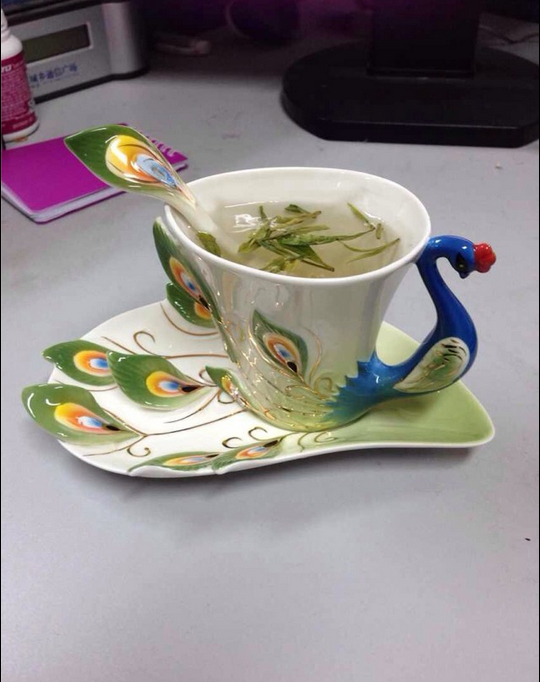
\includegraphics[width=.5\linewidth]{p1}
    % Set English Caption
    \renewcommand{\figurename}{Fig}
    \caption{English title}
    \addtocounter{figure}{-1}
    \vspace{-11pt}
    % Set Chinses Caption
    \renewcommand{\figurename}{图}
    \caption{中文标题}
  \end{minipage}
\end{figure}
\end{minted}
\begin{figure}[htbp]
\begin{minipage}{.5\linewidth}\centering
	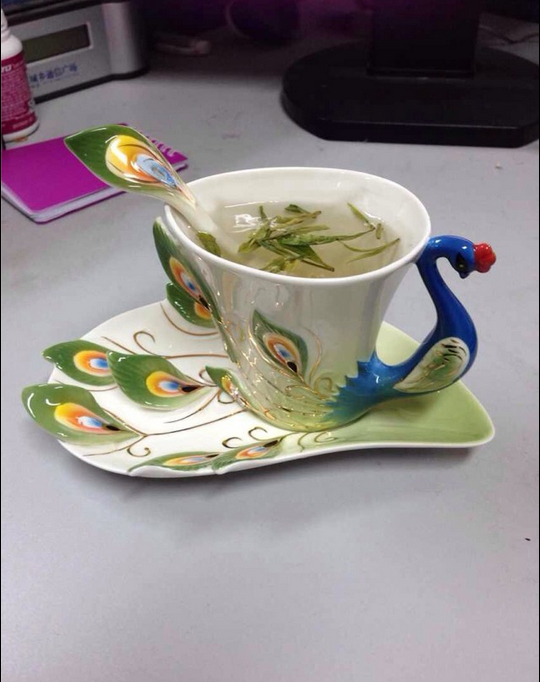
\includegraphics[width=.5\linewidth]{p1}
	\caption{中文标题}
	\addtocounter{figure}{-1}
	\vspace{-11pt}
	% Set English Caption
	\renewcommand{\figurename}{Fig}
	\caption{English title}
\end{minipage}%
\begin{minipage}{.5\linewidth}\centering
	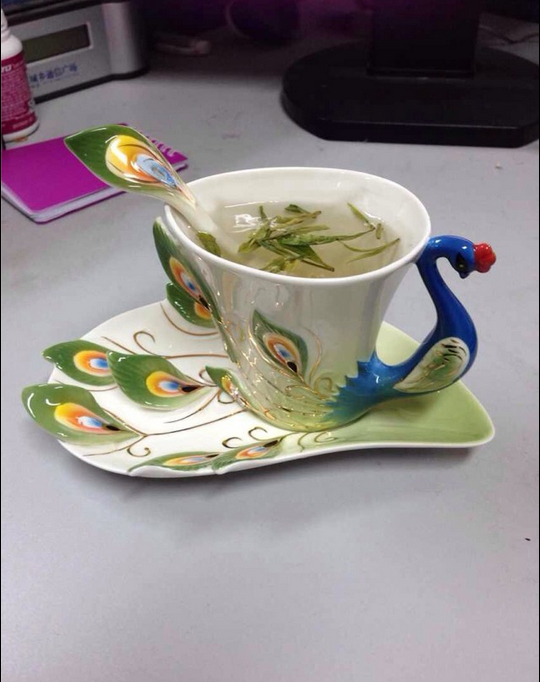
\includegraphics[width=.5\linewidth]{p1}
	% Set English Caption
	\renewcommand{\figurename}{Fig}
	\caption{English title}
	\addtocounter{figure}{-1}
	\vspace{-11pt}
	% Set Chinses Caption
	\renewcommand{\figurename}{图}
	\caption{中文标题}
\end{minipage}
\end{figure}

还可以使用 ccaption 宏包的双语标题 \mt{\bicaption} 命令。
\begin{minted}[xleftmargin=1cm]{tex}
\bicaption[<label>]{<short-1>}{<long-1>}{<NAME>}{<long-2>}
\end{minted}

可选项\mt{<label>}提供交叉引用需要的标签。
\mt{<short-1>}和\mt{<long-1>}分别是短标题和长标题。
\mt{<NAME>}提供第二种语言的标题名,\mt{<long-2>}提供第二种语言的标题内容。

\begin{minted}[xleftmargin=1cm]{tex}
\begin{figure}[htbp]
  \begin{minipage}{.5\linewidth}
    \centering
    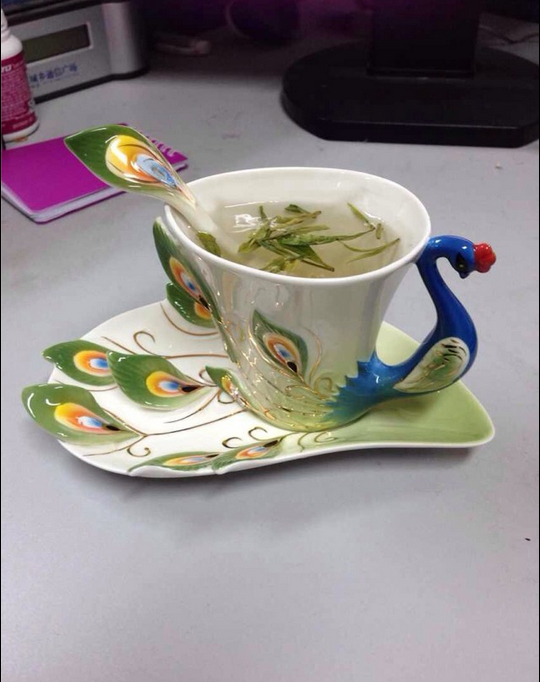
\includegraphics[width=.5\linewidth]{p1}
    \bicaption{ }{中文标题}{Fig}{English title}
  \end{minipage}%
  \begin{minipage}{.5\linewidth}
    \renewcommand{\figurename}{Fig}
    \centering
    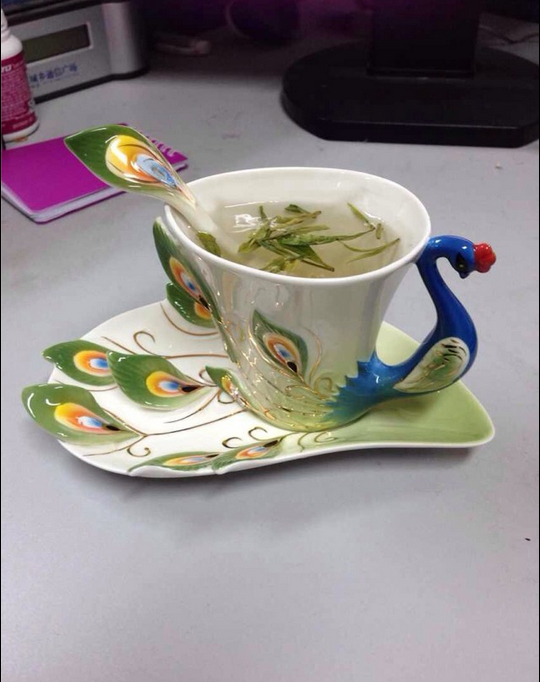
\includegraphics[width=.5\linewidth]{p1}
    \bicaption{ }{English title}{图}{中文标题}
  \end{minipage}
\end{figure}
\end{minted}
\begin{figure}[htbp]
\begin{minipage}{.5\linewidth}
  \centering
  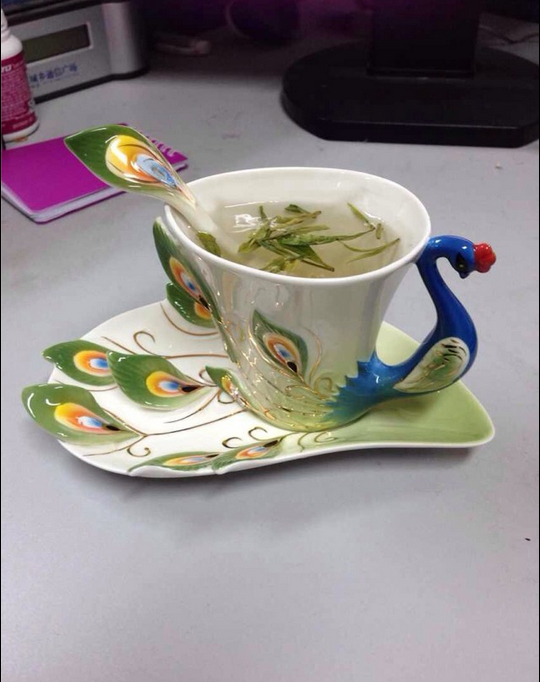
\includegraphics[width=.5\linewidth]{p1}
  \bicaption{ }{中文标题}{Fig}{English title}
\end{minipage}%
\begin{minipage}{.5\linewidth}
  \renewcommand{\figurename}{Fig}
  \centering
  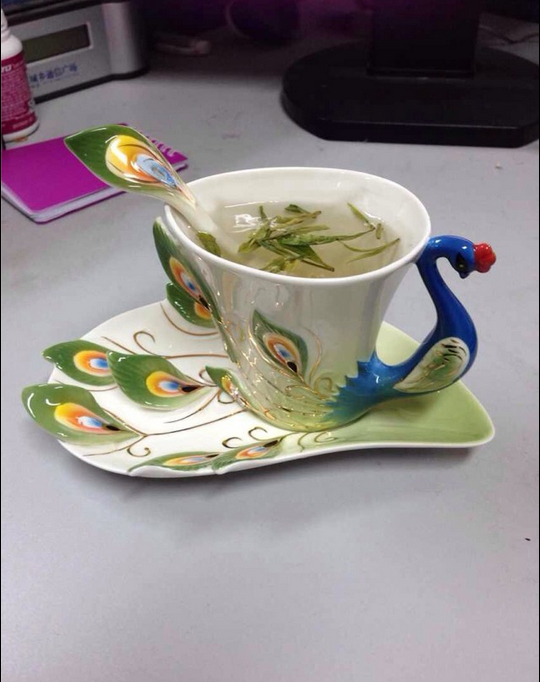
\includegraphics[width=.5\linewidth]{p1}
  \bicaption{ }{English title}{图}{中文标题}
\end{minipage}
\end{figure}

\nocite{*}
\begin{thebibliography}{99}
	\bibitem{ltx225} \LaTeX\_Fun. \emph{\LaTeX{} 技巧225:图表中英文双标题的使用技巧}.  \url{http://blog.sina.com.cn/s/blog_5e16f1770100gvt9.html}
	\bibitem{ccaption} Peter Wilson, Herries Press. \emph{ccaption 宏包手册}.  \url{ftp://ctan.tug.org/tex-archive/macros/latex/contrib/ccaption/ccaption.pdf}
\end{thebibliography}
\end{document}